% Thesis Figure 3.8: multivariate GAN pipeline for SWaT, drawn as a training lane and a
% scoring lane. Method: internal GAN-SWaT report, Sections 2.3.5 and 4.1-4.5, with the
% accompanying tulog/tadgan.py and tulog/main.py; TadGAN (Geiger et al. 2020), Section III.
% Lane (a): the data critic separates observed windows X from G(z), generated from prior
% samples z ~ N(0, I); the latent critic separates z from the encodings E(X).
% Lane (b): only the reconstruction error and the data-critic output on the observed
% window enter the score a_t (Equation 3.1); the latent critic is not used.
% D-055: chronological partition. The first 56,240 attack-period timestamps, with separate
% portions of the normal recording, supply training and validation; the later 393,679 form the
% test set. Validation data select the representation, the settings and the threshold.
% Section 3.5.2: the window is fixed at w = 60 with step 1; only the representation varies.
% PCA uses 5 or 24 components; scaler and PCA fit training data only and are reused.
% Geometry is in millimetres with y pointing down; 140 mm fits the text block.
% lmodern is loaded before the shared style so that math scales to the small sizes used
% here; the style then sets the text face to TeX Gyre Heros as in the other SWaT figures.
\documentclass[border=1pt]{standalone}
\usepackage{lmodern}
% Shared typography and palette for the three corrected SWaT context figures.
% Geometry is in millimetres; 140 mm fits the thesis text block at native scale.
\usepackage[T1]{fontenc}
\usepackage{tgheros}
\renewcommand{\familydefault}{\sfdefault}
\usepackage{tikz}
\usetikzlibrary{calc,patterns}
\definecolor{swatblue}{HTML}{0065BD}
\definecolor{swatlight}{HTML}{98C6EA}
\definecolor{swatgrey}{HTML}{666666}
\tikzset{every node/.style={font=\fontsize{8}{10}\selectfont},
  panel/.style={draw=black!30,fill=white,line width=0.4pt},
  stage/.style={draw=swatblue,fill=swatblue,text=white,align=center,
    minimum height=10mm,text width=19mm,inner sep=0.5mm},
  smalllabel/.style={font=\fontsize{7}{8.5}\selectfont,text=swatgrey}}

\usetikzlibrary{arrows.meta}
\definecolor{tumorange}{HTML}{E37222}
\newcommand{\fT}{\fontsize{7.5}{9}\selectfont\bfseries}
\newcommand{\fH}{\fontsize{7}{8.4}\selectfont\bfseries}
\newcommand{\fB}{\fontsize{7}{8.4}\selectfont\mdseries}
\newcommand{\fS}{\fontsize{6.5}{7.8}\selectfont\mdseries}
\newcommand{\fX}{\fontsize{6}{7.2}\selectfont\mdseries}
\newcommand{\fM}{\fontsize{9}{10}\selectfont}
\begin{document}
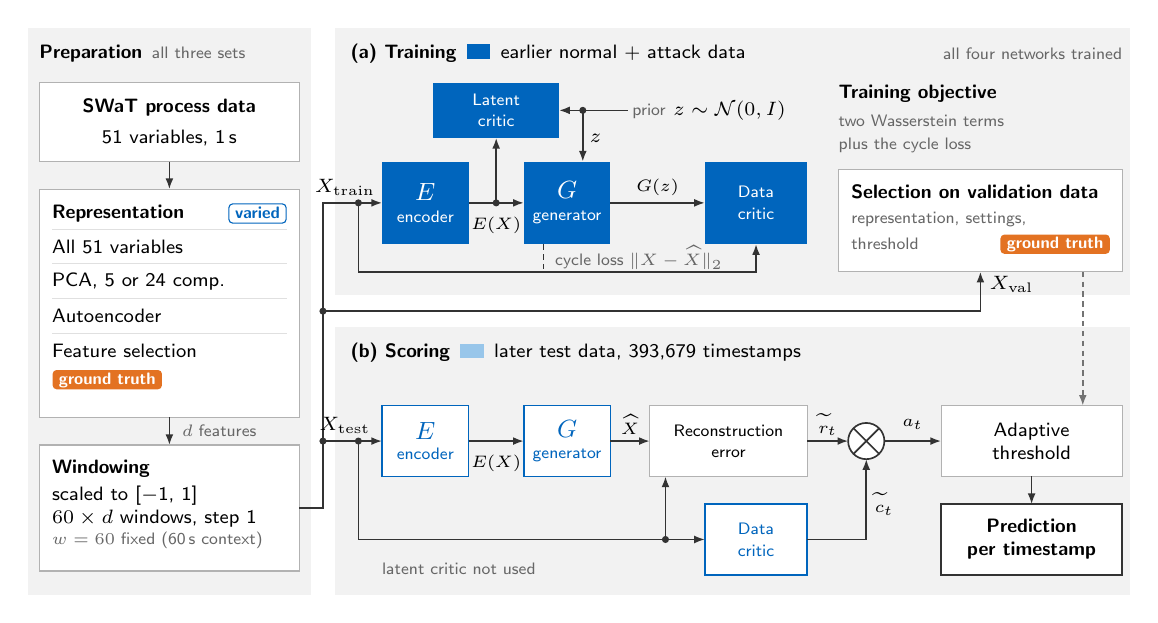
\begin{tikzpicture}[x=1mm,y=-1mm,
    txt/.style={inner sep=0pt,outer sep=0pt},
    op/.style={draw=black!30,fill=white,line width=0.4pt},
    net/.style={fill=swatblue},
    netout/.style={draw=swatblue,fill=white,line width=0.6pt},
    outbox/.style={draw=black!80,fill=white,line width=0.6pt},
    lnk/.style={draw=black!80,line width=0.6pt},
    arr/.style={lnk,-{Latex[length=1.35mm,width=1mm]}},
    dsh/.style={arr,draw=black!55,dash pattern=on 0.7mm off 0.55mm},
    dot/.style={fill=black!80},
    tag/.style={rounded corners=0.5mm,inner xsep=0.8mm,inner ysep=0.35mm,
      text height=1.45mm,text depth=0.3mm,font=\fX\bfseries},
    varied/.style={tag,draw=swatblue,line width=0.4pt,fill=white,text=swatblue},
    labels/.style={tag,fill=tumorange,text=white}]
  \path[use as bounding box] (0,0) rectangle (140,72);

  % Panels
  \fill[black!5] (0,0) rectangle (36,72);
  \fill[black!5] (39,0) rectangle (140,34);
  \fill[black!5] (39,38) rectangle (140,72);

  % Preparation, applied to the training, validation and test sets
  \node[txt,anchor=west] at (1.5,3.3)
    {\fT Preparation\hspace{1.2mm}{\fS\color{swatgrey}all three sets}};
  \draw[op] (1.5,7) rectangle (34.5,17);
  \node[txt,align=center] at (18,12)
    {{\fT SWaT process data}\\[0.4mm]{\fB 51 variables, 1\,s}};
  \draw[arr] (18,17) -- (18,20.5);

  \draw[op] (1.5,20.5) rectangle (34.5,49.5);
  \node[txt,anchor=west] at (3.1,23.6) {\fH Representation};
  \node[varied,anchor=east] at (32.9,23.6) {varied};
  \foreach \y in {25.6,30.0,34.4,38.8}
    \draw[black!12,line width=0.3pt] (3.1,\y) -- (32.9,\y);
  \node[txt,anchor=west] at (3.1,27.8) {\fB All 51 variables};
  \node[txt,anchor=west] at (3.1,32.2) {\fB PCA, 5 or 24 comp.};
  \node[txt,anchor=west] at (3.1,36.6) {\fB Autoencoder};
  \node[txt,anchor=west] at (3.1,41.0) {\fB Feature selection};
  \node[labels,anchor=west] at (3.1,44.7) {ground truth};
  \draw[arr] (18,49.5) -- (18,53);
  \node[txt,anchor=west,text=swatgrey] at (19.6,51.25) {\fS$d$ features};

  % Windowing: the window length is fixed, so it carries no "varied" tag
  \draw[op] (1.5,53) rectangle (34.5,69);
  \node[txt,anchor=west] at (3.1,56.0) {\fH Windowing};
  \node[txt,anchor=west] at (3.1,59.4) {\fB scaled to [$-$1, 1]};
  \node[txt,anchor=west] at (3.1,62.3) {\fB$60\times d$ windows, step 1};
  \node[txt,anchor=west,text=swatgrey] at (3.1,65.1) {\fS$w=60$ fixed (60\,s context)};

  % Bus into the two lanes and the validation branch
  \draw[arr] (34.5,61) -- (37.5,61) -- (37.5,22.25) -- (45,22.25);
  \draw[arr] (37.5,52.5) -- (45,52.5);
  \fill[dot] (37.5,52.5) circle[radius=0.45mm];
  \draw[arr] (37.5,36) -- (121,36) -- (121,31);
  \fill[dot] (37.5,36) circle[radius=0.45mm];
  \node[txt] at (40.3,20.3) {\fontsize{7.5}{9}\selectfont$X_{\mathrm{train}}$};
  \node[txt] at (40.3,50.55) {\fontsize{7.5}{9}\selectfont$X_{\mathrm{test}}$};
  \node[txt,anchor=west] at (122.2,32.6) {\fontsize{7.5}{9}\selectfont$X_{\mathrm{val}}$};

  % (a) Training on earlier normal and attack windows
  \node[txt,anchor=west] at (41,3.3) {\fT (a) Training\hspace{1.3mm}%
    \textcolor{swatblue}{\rule{3mm}{1.8mm}}\hspace{1.3mm}{\fB earlier normal + attack data}};
  \node[txt,anchor=east,text=swatgrey] at (139,3.3) {\fS all four networks trained};

  \fill[net] (51.5,7) rectangle (67.5,14);
  \node[txt,align=center,text=white,font=\fS] at (59.5,10.5) {Latent\\critic};
  \node[txt,anchor=west] at (76.8,10.5)
    {{\fS\color{swatgrey}prior}\hspace{1mm}{\fB$z\sim\mathcal{N}(0,I)$}};
  \draw[arr] (76.2,10.5) -- (67.5,10.5);
  \fill[dot] (70.5,10.5) circle[radius=0.45mm];
  \draw[arr] (70.5,10.5) -- (70.5,17);
  \node[txt,anchor=west] at (71.4,14.1) {\fB$z$};

  \fill[net] (45,17) rectangle (56,27.5);
  \node[txt,align=center,text=white,font=\fX] at (50.5,22.25) {{\fM$E$}\\[0.3mm]encoder};
  \fill[net] (63,17) rectangle (74,27.5);
  \node[txt,align=center,text=white,font=\fX] at (68.5,22.25) {{\fM$G$}\\[0.3mm]generator};
  \fill[net] (86,17) rectangle (99,27.5);
  \node[txt,align=center,text=white,font=\fS] at (92.5,22.25) {Data\\critic};

  \fill[dot] (42,22.25) circle[radius=0.45mm];
  \draw[arr] (42,22.25) -- (42,31) -- (92.5,31) -- (92.5,27.5);
  \draw[arr] (56,22.25) -- (63,22.25);
  \fill[dot] (59.5,22.25) circle[radius=0.45mm];
  \draw[arr] (59.5,22.25) -- (59.5,14);
  \node[txt] at (59.5,25.1) {\fS$E(X)$};
  \draw[arr] (74,22.25) -- (86,22.25);
  \node[txt] at (80,20.3) {\fS$G(z)$};
  \draw[lnk,dash pattern=on 0.7mm off 0.55mm] (65.5,27.5) -- (65.5,31);
  \node[txt,anchor=west,text=swatgrey] at (67,29.25) {\fX cycle loss $\|X-\widehat{X}\|_2$};

  \node[txt,anchor=west] at (103,8.4) {\fH Training objective};
  \node[txt,anchor=west,text=swatgrey] at (103,11.8) {\fS two Wasserstein terms};
  \node[txt,anchor=west,text=swatgrey] at (103,15.0) {\fS plus the cycle loss};

  % Model selection on the validation set
  \draw[op] (103,18) rectangle (139,31);
  \node[txt,anchor=west] at (104.6,20.9) {\fH Selection on validation data};
  \node[txt,anchor=west,text=swatgrey] at (104.6,24.3) {\fS representation, settings,};
  \node[txt,anchor=west,text=swatgrey] at (104.6,27.5) {\fS threshold};
  \node[labels,anchor=east] at (137.5,27.5) {ground truth};
  \draw[dsh] (134,31) -- (134,48);

  % (b) Scoring of the later test set
  \node[txt,anchor=west] at (41,41.3) {\fT (b) Scoring\hspace{1.3mm}%
    \textcolor{swatlight}{\rule{3mm}{1.8mm}}\hspace{1.3mm}{\fB later test data, 393,679 timestamps}};

  \draw[netout] (45,48) rectangle (56,57);
  \node[txt,align=center,text=swatblue,font=\fX] at (50.5,52.5) {{\fM$E$}\\[0.1mm]encoder};
  \draw[netout] (63,48) rectangle (74,57);
  \node[txt,align=center,text=swatblue,font=\fX] at (68.5,52.5) {{\fM$G$}\\[0.1mm]generator};
  \draw[op] (79,48) rectangle (99,57);
  \node[txt,align=center,font=\fS] at (89,52.5) {Reconstruction\\error};
  \draw[netout] (86,60.5) rectangle (99,69.5);
  \node[txt,align=center,text=swatblue,font=\fS] at (92.5,65) {Data\\critic};

  \fill[dot] (42,52.5) circle[radius=0.45mm];
  \draw[arr] (42,52.5) -- (42,65) -- (86,65);
  \fill[dot] (81,65) circle[radius=0.45mm];
  \draw[arr] (81,65) -- (81,57);
  \draw[arr] (56,52.5) -- (63,52.5);
  \node[txt] at (59.5,55.35) {\fS$E(X)$};
  \draw[arr] (74,52.5) -- (79,52.5);
  \node[txt] at (76.5,50.4) {\fS$\widehat{X}$};
  \node[txt,anchor=west,text=swatgrey] at (45,68.7) {\fS latent critic not used};

  \draw[lnk,fill=white] (106.5,52.5) circle[radius=2.3mm];
  \draw[lnk] (104.87,50.87) -- (108.13,54.13) (104.87,54.13) -- (108.13,50.87);
  \draw[arr] (99,52.5) -- (104.2,52.5);
  \node[txt] at (101.6,50.4) {\fS$\widetilde{r}_t$};
  \draw[arr] (99,65) -- (106.5,65) -- (106.5,54.8);
  \node[txt,anchor=west] at (107.6,60.5) {\fS$\widetilde{c}_t$};
  \draw[arr] (108.8,52.5) -- (116,52.5);
  \node[txt] at (112.4,50.4) {\fS$a_t$};

  \draw[op] (116,48) rectangle (139,57);
  \node[txt,align=center,font=\fB] at (127.5,52.5) {Adaptive\\threshold};
  \draw[arr] (127.5,57) -- (127.5,60.5);
  \draw[outbox] (116,60.5) rectangle (139,69.5);
  \node[txt,align=center,font=\fB\bfseries] at (127.5,65) {Prediction\\per timestamp};
\end{tikzpicture}
\end{document}
